\section{Contributions}

% nous allons trouver un compromis entre le temps d'execution et l'equilibrage de charge
%\begin{frame}
%\centering
%	\vspace{2.2cm}       
%	\Huge 
%	\textbf{Pourquoi \\la réduction des transitions externes \\et\\ l'équilibrage des états \\n'aide pas le model checking ?}	
%\end{frame}

% avant tout, presentons les point de partitions
%tout partition outre les point que la formule n'est pas verifier initialement entrainera un nombre de calcule. les exemples precedents le demontre.

%il peut arriver que les machine ne peuvent pas supporter ces etats par leur nombres
%le mieux est de le surcharger en calcule ou en stockage que les deux en meme temps
\subsection{Points de partitions}
\begin{frame}{Définition}
  \centering
   \begin{columns}
   	\begin{column}{0.8\textwidth}
   		\vspace{-20pt}
   		\begin{figure}				
   			\begin{tikzpicture}		
   			\only<1-1>
   			{
   				\node [inner sep=-10pt]
   				{
   					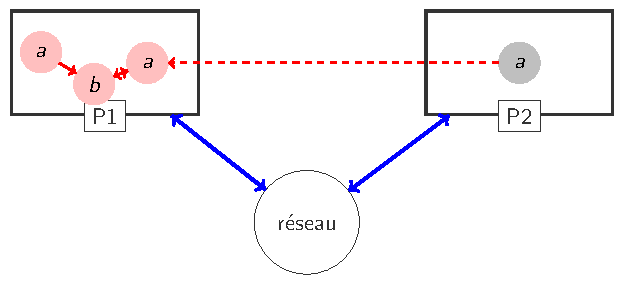
\includegraphics[height=1.2in,width=\columnwidth,trim={0 0 0 0},clip]{resources/benstira/critque1}
   				};              
   			}
   			
   			\node [inner sep=-10pt,visible on=<2->]
   			{
   				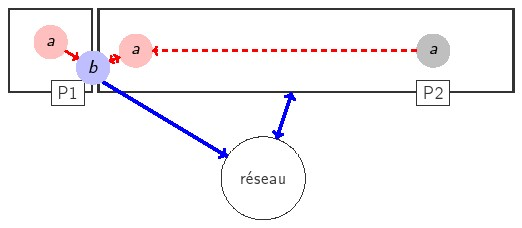
\includegraphics[height=1.2in,width=\columnwidth,trim={0 0 0 0},clip]{resources/pointpartition}
   			};
   		
   			\end{tikzpicture}				
   		\end{figure}
   	\end{column}   	
   \end{columns}

\begin{columns}
	\begin{column}{0.8\textwidth}
		\vspace{15pt}
		\begin{figure}				
			\begin{tikzpicture}	
			\node [inner sep=-10pt,visible on=<3->]
			{
				
\includegraphics[height=1in,width=0.5\columnwidth,trim={0 0 0 0},clip]{resources/pc}
			};			
			\end{tikzpicture}				
		\end{figure}
	\end{column}   	
\end{columns}
\end{frame}

\subsection{Équilibre de Nash}
\begin{frame}{Définition}
\centering
\vspace{-20pt}
\begin{columns}
	\begin{column}{0.3\textwidth}
		\begin{figure}
			\centering
			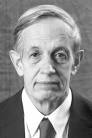
\includegraphics[width=\linewidth]{resources/nash}
		\end{figure}
		
	\end{column}
	\begin{column}{0.7\textwidth}
		\begin{itemize}
			\item Une situation o\`{u} chacun adopte la meilleure réponse du choix des autres.
			\only<2->
			{
			\item Il lui a valu le  \textbf{Prix Nobel}  d'économie en 1994.
			}
			%L'existence d'un équilibre n'implique pas que celui-ci soit nécessairement optimal
		\end{itemize}
	\centering
	\only<3->
	{
		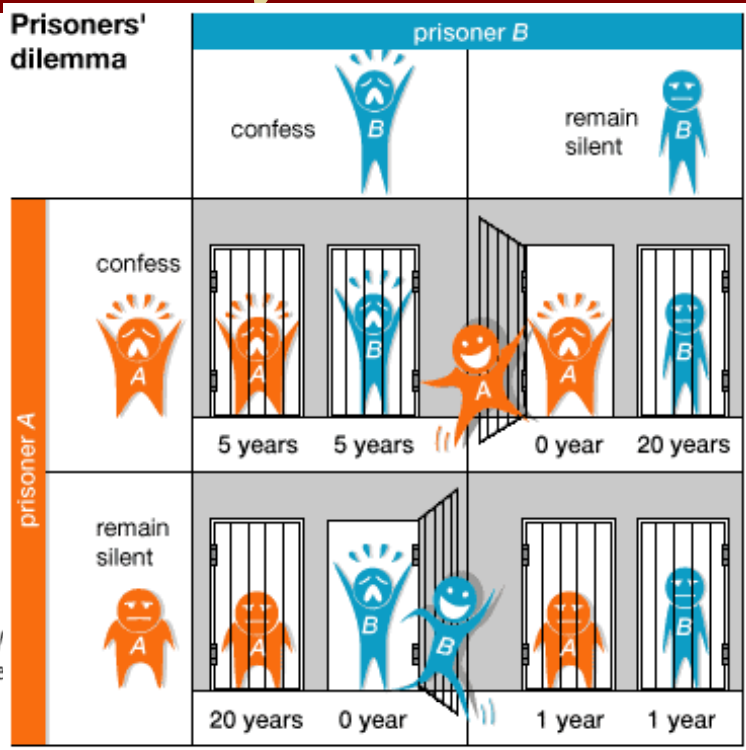
\includegraphics[width=0.5\linewidth]{resources/prisonier}
	}
	\end{column}   	
\end{columns}
\end{frame}


%nous comptons utiliser cette philosophie pour equilibrer le temps de la verification tout en degradant le stockage

\subsection{Stratégie de Distribution}
\begin{frame}{title subsection}

\centering
\vspace{-25pt}
\begin{columns}
	
	\begin{column}{1\textwidth}
		\begin{figure}
			\centering
			\begin{tikzpicture}	
			\node [inner sep=-10pt,visible on=<1-1>]
			{
				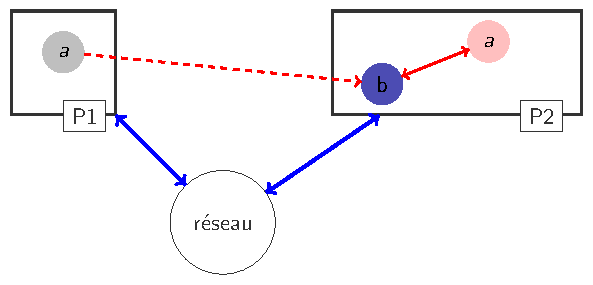
\includegraphics[width=\columnwidth,trim={0 0 0 0},clip]{resources/d1}
			};	
			\node [inner sep=-10pt,visible on=<2-2>]
			{
				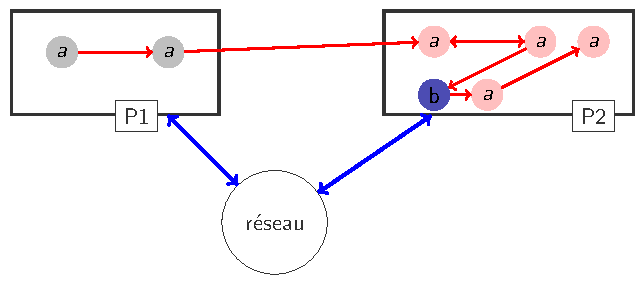
\includegraphics[width=\columnwidth,trim={0 0 0 0},clip]{resources/d3}
			};
	
			\node [inner sep=-10pt,visible on=<3-3>]
			{
				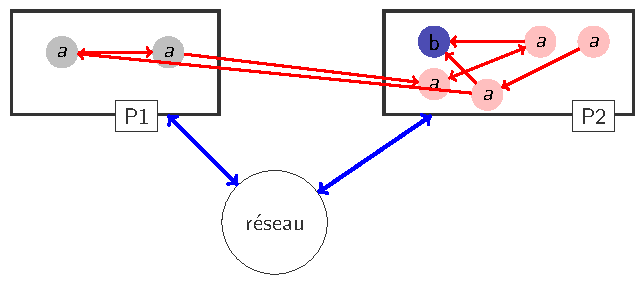
\includegraphics[width=\columnwidth,trim={0 0 0 0},clip]{resources/d2}
			};			
			 
			 	
		 	 \node [inner sep=-10pt,visible on=<4-4>]
		 	{
		 		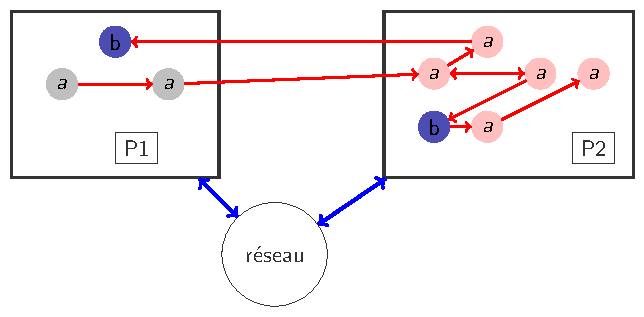
\includegraphics[width=\columnwidth,trim={0 0 0 0},clip]{resources/d4}
		 	};	
			 \node [inner sep=-10pt,visible on=<5-5>]
			 {
			 	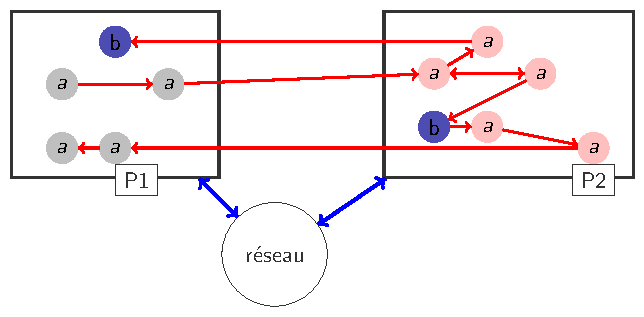
\includegraphics[width=\columnwidth,trim={0 0 0 0},clip]{resources/d6}
			 };
	 
		 	\node [inner sep=-10pt,visible on=<6-6>]
		 	{
		 		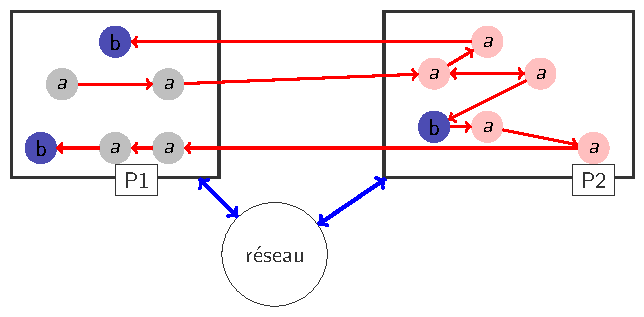
\includegraphics[width=\columnwidth,trim={0 0 0 0},clip]{resources/d5}
		 	};	
	
     	
     		\node [inner sep=-10pt,visible on=<7-7>]
     		{
     			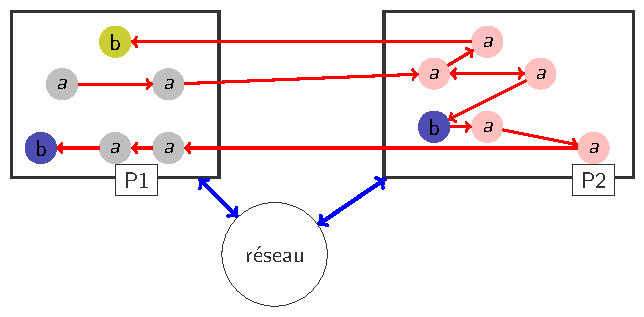
\includegraphics[width=\columnwidth,trim={0 0 0 0},clip]{resources/d7}
     		};	
     	
     		\node [inner sep=-10pt,visible on=<8->]
     		{
     			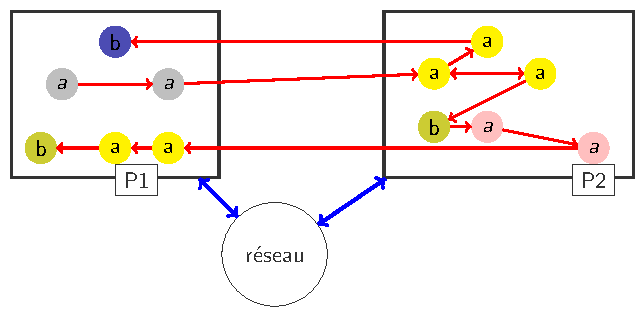
\includegraphics[width=\columnwidth,trim={0 0 0 0},clip]{resources/d8}
     		};	
     	
			\end{tikzpicture}
		\end{figure}		
	\end{column} 
	
\end{columns}
\end{frame}
%nous comptons a realiser une meilleur partion
\subsection{Model checking par déduction}
\begin{frame}{title subsection}
	\begin{block}
	
	\begin{itemize}
		\item Notion de duplicata
		\item Déduit la valeur logique des duplicatas
		\item Minimise le taux de communications
	\end{itemize}
	\end{block}
\end{frame}

%ces deux approche permet d'accelerer le temps de la verification d'une propriete 

\subsection{Exemple}
\begin{frame}{Exemple}
	\begin{columns}
		
		\begin{column}{0.4\textwidth}
			\begin{figure}
				\centering
				\only<1-1>
				{ 
					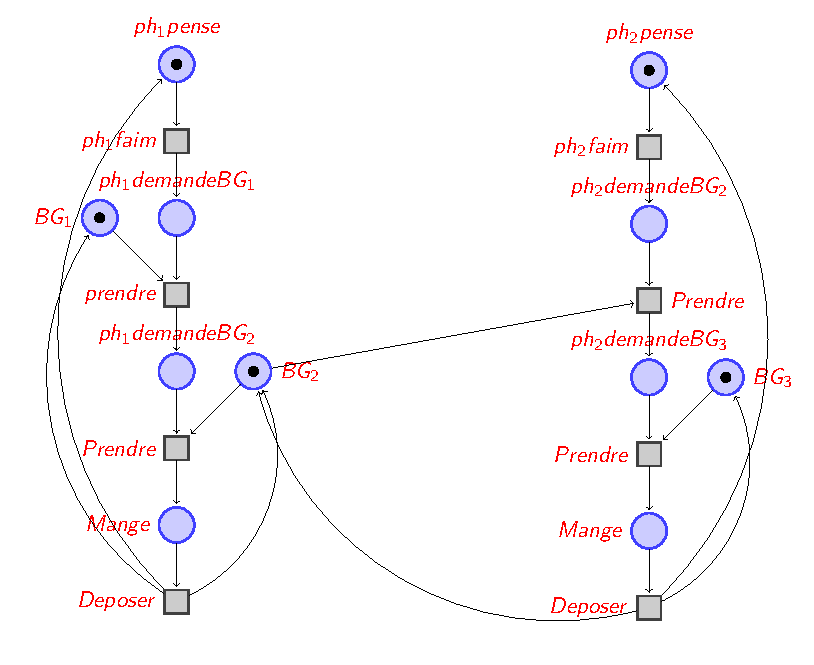
\includegraphics[width=\linewidth]{resources/testpetri1}
				}
				\only<2-2>
				{
					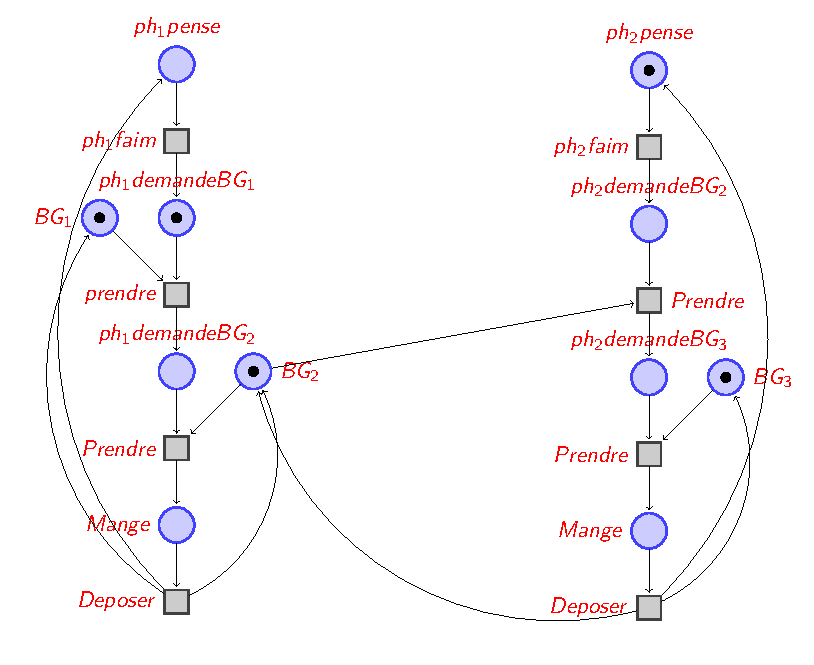
\includegraphics[width=\linewidth]{resources/testpetri2}
				}
				\only<3-3>
				{
					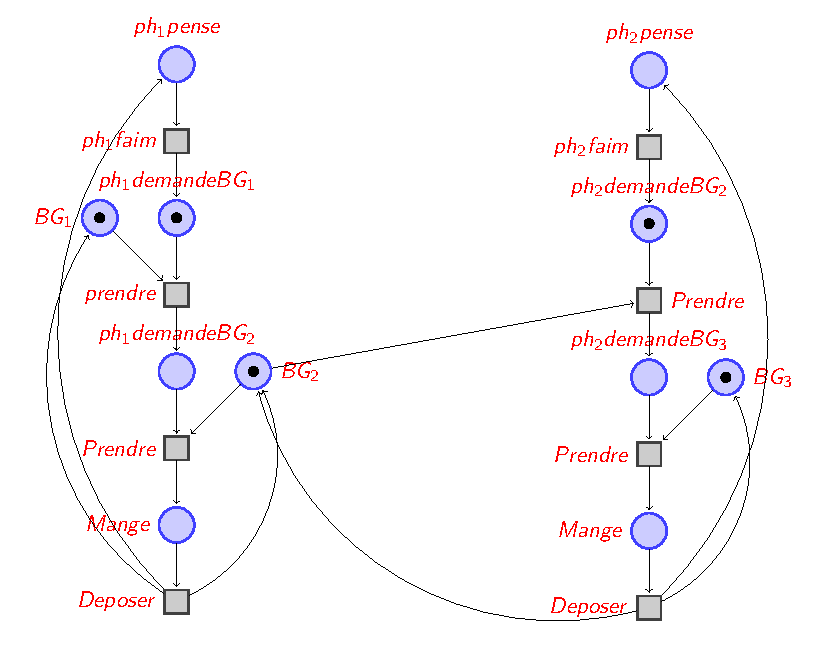
\includegraphics[width=\linewidth]{resources/testpetri3}
				}
				\only<4-4>
				{
					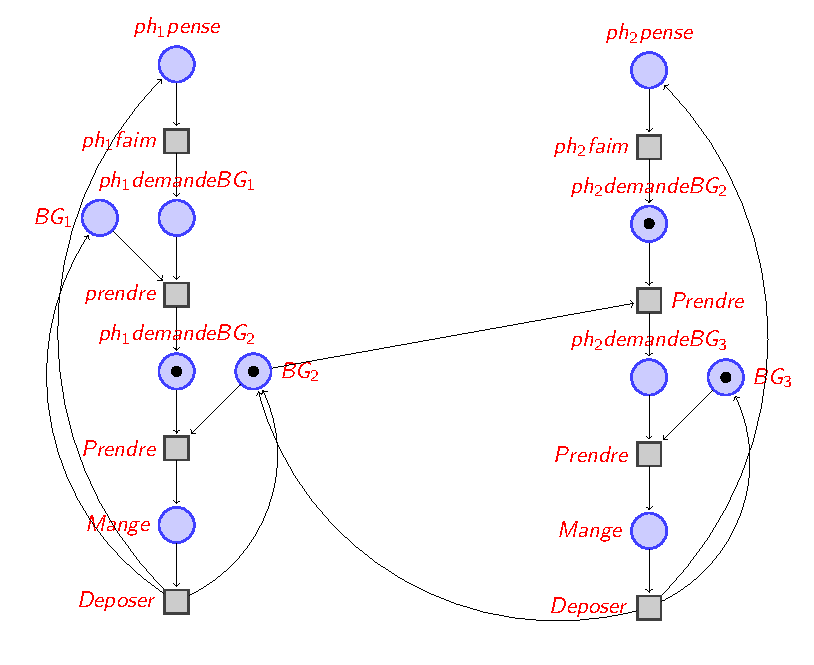
\includegraphics[width=\linewidth]{resources/testpetri4}
				}
				\only<5-5>
				{
					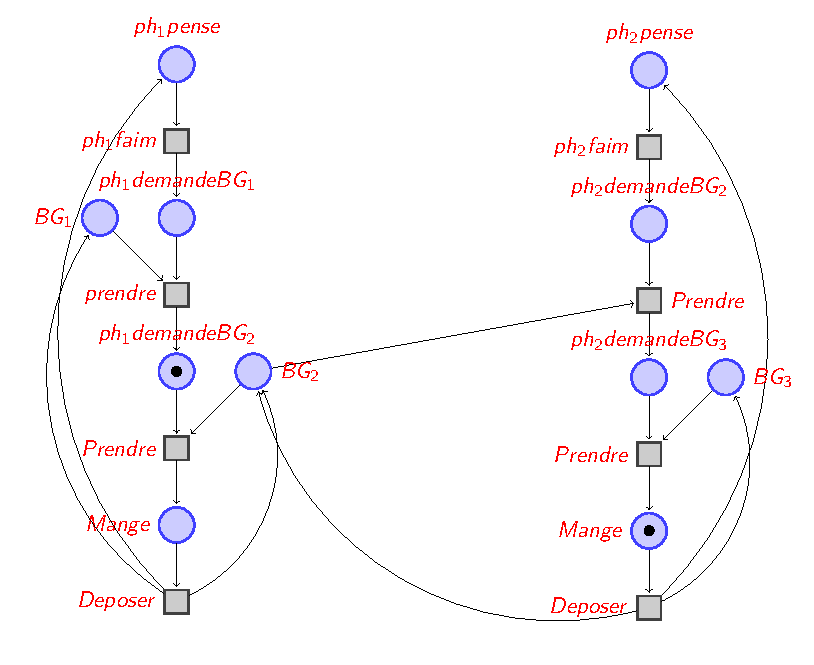
\includegraphics[width=\linewidth]{resources/testpetri5}
				}
				\only<6-6>
				{
					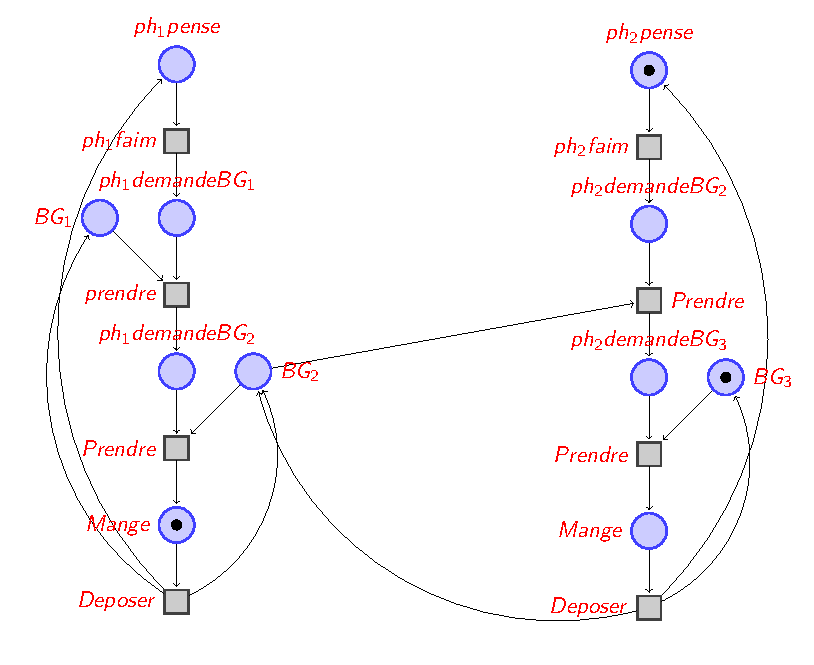
\includegraphics[width=\linewidth]{resources/testpetri6}
				}
				\only<7->
				{
					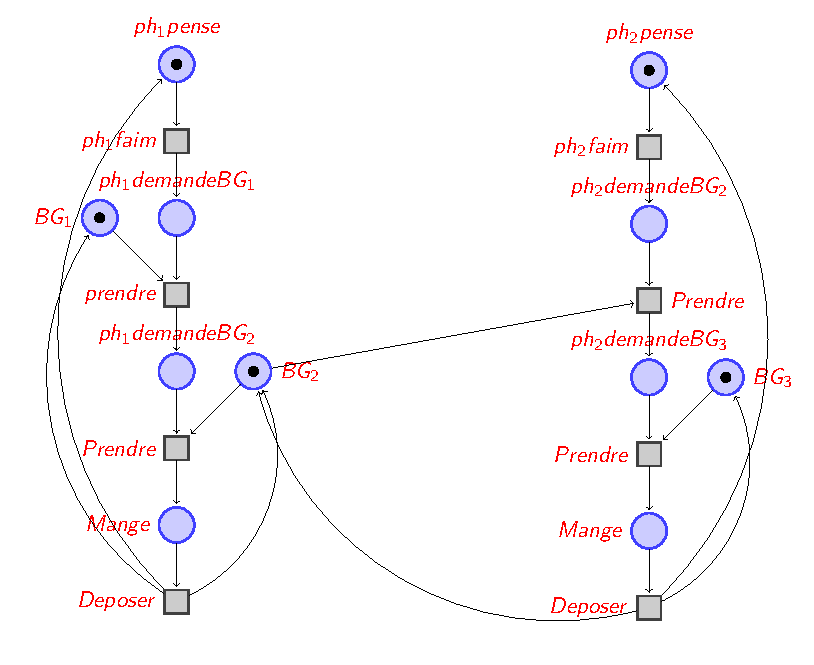
\includegraphics[width=\linewidth]{resources/testpetri7}
				}
			\end{figure}			
		\end{column}
	
		\begin{column}{0.5\textwidth}
			\begin{figure}
				\centering
				\only<7-8>
				{
					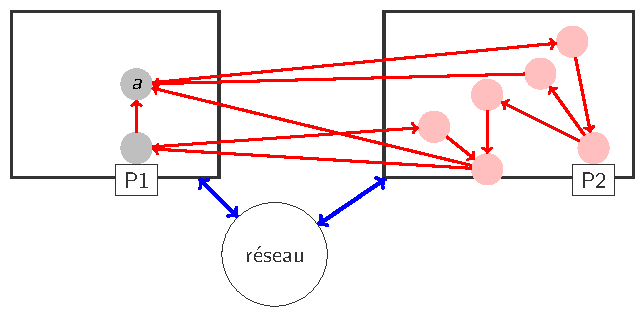
\includegraphics[width=\linewidth]{resources/DRDP1}
				}
				\only<9-9>
				{
					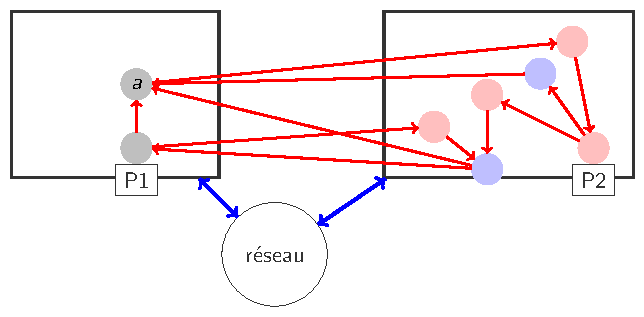
\includegraphics[width=\linewidth]{resources/DRDP2}
				}
				
			\end{figure}			
		\end{column}
	\end{columns}
\end{frame}


\subsection{Résultat}
\begin{frame}{Exemple}

\begin{columns}
	\begin{column}{0.9\textwidth}
		\begin{figure}
			\vspace{-25pt}
			\centering
			
		\begin{tikzpicture}[scale=0.6]
			\draw[thick,<->] (0,8) node[right]{Temps d'exécution}--(0,0)--(14,0) node[right]{Formule CTL};
			
			\only<1->
			{
			\draw [blue](0,5)--(2,5);
			}
			\only<2->
			{
			\draw [blue](2,7)--(3,7);
			}
			\only<3->
			{
			\draw [blue](3,4)--(5,4);
			}
			\only<4->
			{
			\draw [blue](5,3)--(8,3);
			}
			\only<5->
			{
			\draw [blue](8,5.5)--(8.5,5.5);
			}
			\only<6->
			{
			\draw [blue](8.5,2)--(14,2);
			}
					
			\node [below] at (1,0) {$f_1$};		
			\node [left] at (0,1) {$t_1$};
			\node [left] at (0,1.5) {$t_2$};
			\node [left] at (0,2) {$t_3$};
			\node [left] at (0,3) {$t_4$};
			\node [left] at (0,5) {$t_5$};
			\node [left] at (0,4) {$t_6$};
			\node [left] at (0,7) {$t_8$};
			\node [left] at (0,5.5) {$t_7$};		
			\node [below] at (0,0) {$f_1$};
			\node [below] at (1,0) {$f_2$};
			\node [below] at (2,0) {$f_3$};
			\node [below] at (3,0) {$f_4$};
			\node [below] at (4,0) {$f_1$};
			\node [below] at (5,0) {$f_2$};
			\node [below] at (6,0) {$f_5$};
			\node [below] at (7,0) {$f_7$};
			\node [below] at (8,0) {$f_2$};
			\node [below] at (9,0) {$f_2$};
			\node [below] at (10,0) {$f_1$};
			\node [below] at (11,0) {$f_2$};
			\node [below] at (12,0) {$f_3$};	
			
			\only<2->
			{	
			\draw[red,dashed](2,5)->(2,7);
			\draw [red, fill=white] (2,5) circle (1.5pt);
			}
			\only<3->
			{				
			
			\draw [green, fill=white] (5,4) circle (1.5pt);
			\draw[green,dashed](3,7)->(3,4);
			
			\draw [green] (3,7) circle (1.5pt);	
			}
			 \only<3->
			 {\draw[green,dashed](5,3)->(5,4);}
 
				\only<5->
			{
				
			\draw[red,dashed](8,3)->(8,5.5);
			\draw [red, fill=white] (8,3) circle (1.5pt);
			}
				\only<6->
			{
			\draw[green,dashed](8.5,5.5)->(8.5,2);	
			\draw [green] (8.5,5.5) circle (1.5pt);	
		}				
			
		\end{tikzpicture}
		\end{figure}			
	\end{column}
\end{columns}
\end{frame}
